\documentclass{article}

% NeurIPS 2025 style, preprint (arXiv-ready). Russian via XeLaTeX + fontspec.
% NOTE: official neurips_2025.sty is *single-column* (textwidth=5.5in).
% For this Russian preprint we override geometry and force a two-column body.
\usepackage[preprint]{neurips_2025}

\usepackage{fontspec}
\usepackage{polyglossia}
\setdefaultlanguage{russian}
\setotherlanguage{english}
\setmainfont{Liberation Serif}
\setsansfont{Liberation Sans}
\setmonofont{Liberation Mono}

\usepackage{amsmath,amssymb}
\usepackage{booktabs}
\usepackage{multirow}
\usepackage{graphicx}
\usepackage{url}
\usepackage{hyperref}
\usepackage{xcolor}
\usepackage{microtype}
\usepackage{enumitem}

\graphicspath{{images/}{../mmcs-sfedu_thesis7/images/}}

% --- Two-column override (must run after neurips_2025 geometry hook) ---
% Official NeurIPS is single-column (5.5in). We widen the text block and
% use \twocolumn[…] for full-width title/abstract + two-column body.
% \@notice uses a float, which is illegal inside \twocolumn's optional
% argument --- replace with a footnote-style notice.
\makeatletter
\renewcommand{\@notice}{%
  \begingroup
    \renewcommand{\thefootnote}{}%
    \footnotetext[0]{\hspace*{-\parindent}\footnotesize\@noticestring}%
  \endgroup
}
\AtBeginDocument{%
  \newgeometry{%
    letterpaper,%
    textheight=9in,%
    textwidth=7in,%
    top=1in,%
    left=0.75in,%
    headheight=12pt,%
    headsep=25pt,%
    footskip=30pt%
  }%
  \setlength{\columnsep}{0.25in}%
  \setlength{\columnseprule}{0pt}%
}
\makeatother

\newcommand{\rem}{\mathrm{REM}}
\newcommand{\elpd}{\mathrm{elpd}}
\newcommand{\PS}{ПС}

\title{Байесовская точка разладки в динамике парадоксального сна\\
крыс в окрестности сейсмических событий}

\author{%
  С.~А.~Пономарёв \\
  Институт математики, механики и компьютерных наук\\
  Южный федеральный университет \\
  \texttt{ponomarev@sfedu.ru} \\
}

\begin{document}

% Full-width title block + abstract, then two-column body.
\twocolumn[{%
\maketitle
\begin{abstract}
Проверяется гипотеза о статистически различимом изменении динамики
парадоксального сна (ПС,~REM) у крыс за несколько суток до сейсмического
события. По гипнограммам строятся суточные REM-профили; в качестве
признаков используются суточное среднее и \emph{размах профиля ПС}
(классическая нейросейсмологическая метрика). Байесовская модель одной
точки разладки~$\tau$ с маргинализацией дискретного положения оценивается
NUTS; модели сравниваются по PSIS-LOO (\texttt{elpd} на пару
``событие--крыса'').

По двум независимым сеткам предобработки (скользящие окна $W/S$ и
параметризация $N\times\mathrm{overlap}$) апостериорное среднее
$\mathbb{E}[\tau]$ устойчиво лежит в диапазоне $\approx 6{,}5$--$6{,}7$
суток до толчка. Ранжирование признаков по LOO, напротив, зависит от
сетки и семейства правдоподобия: лидерство \texttt{concat:mean} либо
\texttt{daily:range}+plain~beta \emph{не} следует трактовать как
уникальный физиологический вывод. Для bounded-признака размаха plain~Beta
может завышать ELPD из-за плотности у границы~$1$; предпочтительны
constrained~beta / interval-inflated beta либо связка mean+range.
Результат --- свидетельство смены REM-режима, а не прямое измерение
стресса и не прогноз землетрясений.

\medskip
\noindent\textbf{Ключевые слова:}
парадоксальный сон, точка разладки, байесовский вывод, PSIS-LOO,
нейросейсмология.
\end{abstract}
\vspace{1.2em}
}]

\section{Введение}

Геофизические и геохимические предвестники сейсмических событий
описаны для ряда регионов~\cite{Rodkin2011,Cicerone2009,Conti2021}, а
поведенческие аномалии животных перед толчками обсуждаются в
биологической литературе~\cite{Kirschvink2000,Grant2011,Yokoi2003}.
Эти наблюдения сами по себе не задают оперативный предвестник и требуют
проверки на инструментальных физиологических рядах.

Стресс и тревога у грызунов меняют структуру
парадоксального сна~\cite{Rampin1991,Meerlo1997,Palma2000,Sanford2010}.
Парадоксальный сон характеризуется специфической ЭЭГ-картиной и у крыс
входит в выраженный суточный ритм~\cite{Vyazovskiy2005}. Непрерывная
регистрация сна позволяет поставить узкий статистический вопрос: есть
ли смена режима REM-динамики в фиксированном окне до толчка?

Классические нейросейсмологические отчёты по той же площадке опирались
на \emph{размах профиля ПС} по $12$ неперекрывающимся $2$-часовым бинам
и сообщали выраженный эффект в окне \emph{примерно $2$--$4$ суток}
до/после сильных событий (интенсивность $>2$). Здесь мы оцениваем иной
параметр --- момент \emph{начала} нового режима $\tau$ в байесовской
модели одной разладки на восьми сутках до события --- и явно разводим
эти два estimand'а.

Особенность задачи --- сверхмалая выборка, неоднородность животных и
событий, автокорреляция суточных рядов. Это ограничивает ``чёрные
ящики'' и требует явного учёта неопределённости положения разладки.
Работа не направлена на прогноз землетрясений и не измеряет стресс
напрямую (кортикостерон, поведение тревоги не регистрировались).

\section{Данные}

\subsection{Животные и регистрация}

ЭКоГ и электрическая активность гиппокампа непрерывно регистрировались у
взрослых самцов крыс линии пасюк на станции ``Институт'' КФ ЕГС РАН
(Петропавловск-Камчатский). Животных содержали индивидуально при
$23\pm1^{\circ}$C и режиме освещения $12$\,ч свет / $12$\,ч темнота.
Электроды в сенсомоторной коре и поле CA1 гиппокампа соединялись с
$32$-канальной системой; частота оцифровки $1$\,кГц. Процедуры одобрены
биоэтической комиссией ЮФУ.

\subsection{События и окна}

Для анализа отобраны даты с инструментальной интенсивностью $>2$ баллов
и доступной гипнограммой. Базовая диссертационная выборка --- $14$ дат
(2022--2025) и $20$ пар ``событие--крыса'' (две даты 2025\,г.\
представлены четырьмя животными каждая). Июльская перепроверка
использует расширенный экспорт: до $36$ перечисленных окон, из них
$33$ полных восьмидневных профиля в likelihood.

Каждое окно --- \emph{восемь суток} относительно даты события.
Направление \texttt{before} --- пресобытийный ряд (основной estimand
onset). Направление \texttt{after\_reversed} --- послесобытийное окно,
развёрнутое во времени для единого builder'а; биологически ближе к
recovery, часто Pareto-тяжёлое. Неполные \texttt{after\_reversed}
(пропуски суток, \texttt{exported=False}) в LOO не импутируются:
R2~$2024$-$10$-$29$, R3~$2025$-$01$-$23$, R3~$2025$-$03$-$14$.

Профили около $2024$-$09$-$30$ (R2/R3, before и after\_reversed) ---
систематические трудные случаи (высокий Pareto-$k$; для shape-признаков
R2 всегда исключается). Их исключение --- отдельная страта
чувствительности, а не скрытый фильтр.

\section{REM-профили и признаки}

\subsection{Гипнограмма}

Суточную запись разбивают на неперекрывающиеся эпохи $5$\,с. После
исключения артефактов по спектрам мощности медленный сон определяют по
высокой мощности ЭКоГ в дельта-диапазоне $2{,}5$--$5{,}5$\,Гц, а
парадоксальный --- по высокому отношению тета/дельта в
гиппокампе~\cite{Fang2010,Vyazovskiy2005,Saevskiy2025}. Результат ---
гипнограмма с метками бодрствования, медленного и парадоксального сна.

\subsection{Конструкция профиля: $N\times\mathrm{overlap}$}

Суточный REM-профиль --- доли времени в ПС в бинах профиля. Канонические
параметры переписанного пайплайна:
\begin{itemize}[leftmargin=1.4em,itemsep=0.2em,topsep=0.3em]
  \item \texttt{n\_points\_per\_day} $N\in\{12,24,48\}$ (границы $[4,96]$);
  \item \texttt{overlap} $\mathrm{ov}\in\{0,0{,}25,0{,}5\}$ (границы $[0,1)$);
  \item \texttt{rem\_stage}${}=2$.
\end{itemize}
Классическая схема $12\times 2$\,ч без перекрытия эквивалентна
$(N{=}12,\,\mathrm{ov}{=}0)$ и совпадает с доктриной ранних
нейросейсмоотчётов (размах профиля ПС).

Устаревшая параметризация скользящих окон $(W,S)$ (deprecated)
конвертируется:
\[
N=24/S,\qquad
\mathrm{ov}=1-S/W\quad (W>S).
\]
В частности $(W,S)=(2,1)\equiv(N{=}24,\,\mathrm{ov}{=}0{,}5)$ ---
фаворит диссертационной $896$-сетки; $(2,2)\equiv(12,0)$. Окна
$(3,1)$ и $(6,1)$ дают $\mathrm{ov}\approx0{,}67$ и $0{,}83$ и
\emph{не} входят в стандартную июльскую сетку: новая сетка не является
строгим надмножеством старой, но добавляет $N{=}48$ и явную ось
перекрытия.

\subsection{Онтология признаков}

По профилю $P=(p_i)_{i=1}^{N}$ вычисляют суточное среднее
$\bar P=N^{-1}\sum_i p_i$ и размах $R=\max P-\min P$
(\emph{размах профиля ПС} в терминологии old\_neuroseismoreports).
Размах намеренно смешивает экстремумы светлого и тёмного периодов.

Агрегация по сериям чанков (legacy / диссертация):
\texttt{concat}, \texttt{even}, \texttt{odd} $\times$
$\{\texttt{mean},\texttt{range}\}$ --- вектор признаков вдоль окна с
общим $\tau$. Агрегация по суткам (июльский основной запуск):
\texttt{daily} / \texttt{day} / \texttt{night} --- скаляр на сутки
или полусутки; ближе к классическому ``суточный размах''.

Каждый восьмидневный ряд масштабируют в $[0,1]$ независимо для пары
``событие--крыса'' (форма динамики, не абсолютный уровень REM). Для
размаха при Beta-семействе используют \texttt{support\_upper}${}=2$
(наблюдение $R/2$).

Исследовательский блок \texttt{shape\_shift} (L1/L2 динамики формы
профиля, likelihood gamma) в июле даёт слабый/нестабильный сигнал
($\mathbb{E}[\tau]$ часто у нижней границы prior) и не считается
primary.

\begin{figure}[t]
  \centering
  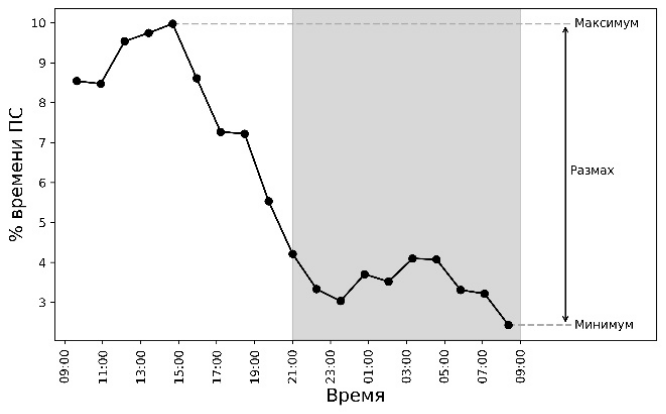
\includegraphics[width=\linewidth]{rem_profile.png}
  \caption{Пример суточного REM-профиля: доли ПС по бинам.
  Классический размах профиля ПС --- разность максимума и минимума.}
  \label{fig:rem-profile}
\end{figure}

\section{Байесовская модель одной разладки}

\subsection{Модель и маргинализация $\tau$}

Для вектора признаков $\mathbf{x}_t$ на сутках $t=1,\ldots,8$ до
события:
\[
\mathbf{x}_t\sim
\begin{cases}
p(\mathbf{x}_t\mid\boldsymbol{\theta}_1), & t<\tau,\\
p(\mathbf{x}_t\mid\boldsymbol{\theta}_2), & t\ge\tau.
\end{cases}
\]
Параметр $\tau$ --- дискретная равномерная априорная величина на
допустимых сутках (типично $\{3,\ldots,8\}$); её маргинализуют из
целевой плотности, после чего применим NUTS~\cite{HoffmanGelman2014,
lai2023automaticallymarginalizedmcmcprobabilistic}. Апостериор
$p(\tau\mid\mathcal{D})$ восстанавливают усреднением условных
вероятностей положений. Параметры режимов $\boldsymbol{\theta}_1$,
$\boldsymbol{\theta}_2$ снабжают слабоинформативными априорными
распределениями (для Beta-форм --- Gamma; для constrained ---
смещение, гарантирующее $\alpha,\beta\ge 1$).

\begin{figure}[t]
  \centering
  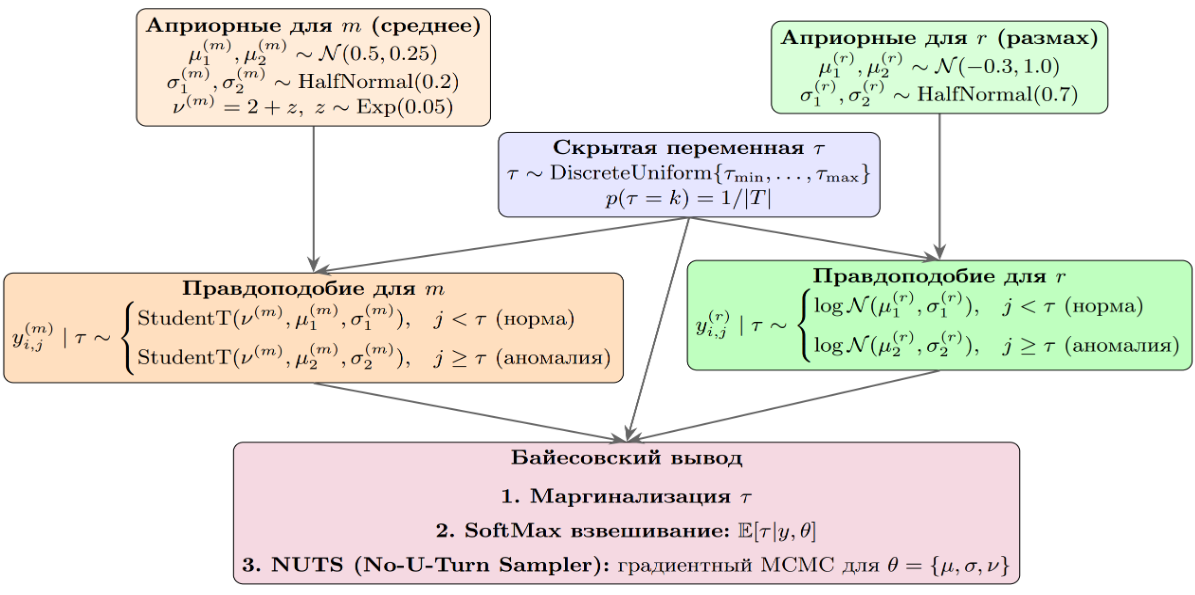
\includegraphics[width=\linewidth]{tau_model.png}
  \caption{Схема модели одной разладки: скрытая $\tau$ разделяет
  фоновый и аномальный режимы; для mean и range --- отдельные
  likelihood/prior.}
  \label{fig:tau-model}
\end{figure}

\subsection{Семейства правдоподобия}

\begin{itemize}[leftmargin=1.4em,itemsep=0.25em,topsep=0.3em]
  \item Среднее: Student-$t$, normal, (в старой сетке также lognormal).
  \item Размах: plain Beta; interval-inflated Beta (IIB, порог
  инфляции $\approx0{,}9$); \texttt{beta\_constrained}
  (те же Beta-наблюдения, но $\alpha,\beta\ge 1$ через
  \texttt{gamma\_offset}).
\end{itemize}
Plain Beta допускает U-образные плотности ($\beta<1$) и при массе
наблюдений у верхней границы даёт взрыв PDF --- см.\ аудит ниже.
Эмпирические диагностики likelihood показывают: для daily-mean
student\_t~$\approx$~normal; для daily-range уместны beta/IIB; для
concat-range часто масса около $0$ (скорее zero-inflated, чем IIB у
верхней границы).

\subsection{Сравнение моделей: ELPD / LOO}

Качество обобщения --- PSIS-LOO~\cite{Vehtari2017,Kumar2019}. Единица
наблюдения --- пара ``событие--крыса'' (внутри события суммируют
поточечный log-lik по суткам/чанкам). Ранжирование --- по
\[
\overline{\elpd}_{\mathrm{LOO}}/(F\cdot E'),
\]
где $F$ --- число активных признаков, $E'$ --- число записей после
возможного исключения влиятельных наблюдений. В тексте дополнительно
уместен $\mathrm{LOO\text{-}IC}=-2\,\widehat{\elpd}_{\mathrm{LOO}}$.

\paragraph{Почему ELPD может быть $>0$.}
Continuous densities --- не вероятности. Для Beta с $\beta<1$ PDF
спайкует при $y\to 1$ и превышает $1$, поэтому log-density положительна.
Сумма таких вкладов даёт положительный $\elpd_{\mathrm{LOO}}$. Это
стандарт ArviZ, а не ошибка знака.

Контроль MCMC: $\hat R\le 1{,}05$, достаточный ESS, отсутствие
дивергенций, диагностика Парето $\hat k$.

\section{Методология поиска}

\subsection{Диссертационный перебор ($896$ конфигураций)}

Варьировали $W\in\{2,3,6\}$\,ч, $S\in\{1,2\}$\,ч, блоки
\texttt{concat}/\texttt{even}/\texttt{odd}${}\times{}$
$\{\texttt{mean},\texttt{range}\}$, likelihoods student\_t / lognormal /
beta. Каждая модель: $4$ цепи, $3000$ tune + $1000$ draws. Все
$896$ прошли критерии сходимости. Распределение нормированного ELPD
имело плато основной массы и выделенный верхний хвост; центральная
часть близка к нормальному закону ($\mu\approx 3{,}20$,
$\sigma\approx 1{,}01$, $R^2_{\mathrm{QQ}}\approx 0{,}975$).

\begin{table}[t]
\centering
\caption{Доля REM-признаков в квартилях ELPD ($896$-сетка), \%.
Q1 --- лучший квартиль.}
\label{tab:feat-q}
\small
\begin{tabular}{lrrrr}
\toprule
Признак & Q1 & Q2 & Q3 & Q4\\
\midrule
\texttt{concat:mean}  & 94 & 80 & 40 & 0\\
\texttt{concat:range} & 53 & 54 & 62 & 45\\
\texttt{even:mean}    & 47 & 54 & 63 & 50\\
\texttt{odd:mean}     & 43 & 55 & 62 & 54\\
\texttt{even:range}   & 27 & 58 & 60 & 69\\
\texttt{odd:range}    & 38 & 55 & 60 & 62\\
\bottomrule
\end{tabular}
\end{table}

Средний нормированный ELPD для $W{=}2$\,ч составлял
$3{,}46\pm1{,}07$ против $2{,}65\pm0{,}72$ для $W{=}6$\,ч; шаг $S$
почти не влиял ($3{,}18$ vs $3{,}23$). Признак \texttt{concat:mean}
встречался в $94\%$ моделей Q1 и во всех лучших $5\%$ (точный критерий
Фишера, $p<0{,}001$). Добавление \texttt{range} сужало апостериор
$\tau$ в $1{,}3$--$1{,}9$ раза, но ухудшало ELPD --- компромисс
локализации и предсказательной способности. Эти цифры описывают
\emph{структуру одной сетки}; они не переносятся как уникальный
физиологический ранг на июльский builder.

\subsection{Июльский перебор ($N\times\mathrm{overlap}$)}

Основной запуск: $N\in\{12,24,48\}\times\mathrm{ov}\in\{0,0{,}25,0{,}5\}$,
$1224$ завершённых конфигурации ($1079$ eligible для ранжирования),
daily/day/night агрегаты, mean $\in\{\texttt{student\_t},\texttt{normal}\}$,
range $\in\{\texttt{beta},\texttt{interval\_inflated\_beta}\}$. Отдельно ---
абляция shape\_shift ($126$ конфигов). Длинные refits топ-моделей
(tune~$6000$, draws~$3000$) подтверждают костяк ранжирования внутри
июльского builder'а.

\begin{table}[t]
\centering
\caption{Фрагмент top-eligible июля (plain beta на range ---
диагностический срез; см.\ аудит границы).}
\label{tab:july-top}
\small
\begin{tabular}{cllcrr}
\toprule
\# & Признаки & Lik. & $N$/ov & ELPD/$F E'$ & $\mathbb{E}[\tau]$\\
\midrule
1 & daily:range & beta & 48/0 & $6{,}63$ & $6{,}28$\\
2 & daily:range & beta & 48/0.5 & $6{,}24$ & $7{,}98$\\
4 & daily:m+r & $t$+beta & 48/0 & $6{,}03$ & $6{,}47$\\
5 & daily:m+r & n+beta & 48/0 & $5{,}99$ & $6{,}80$\\
\bottomrule
\end{tabular}
\end{table}

В top-$50$: \texttt{daily:mean+range} ($28$), \texttt{day:range} ($15$),
\texttt{daily:range} ($14$), \texttt{daily:mean} ($8$); likelihood
range${=}beta$ ($34$), mean${=}normal$ ($22$), mean${=}student\_t$ ($17$),
IIB ($11$). Разрешение $N{=}48$, $\mathrm{ov}{=}0$ доминирует
($26/50$); грубое $N{=}12$ почти не попадает в верх. Shape-shift:
лучший ELPD/feat отрицательный ($\approx -6{,}4$),
$\mathbb{E}[\tau]_{\mathrm{top20}}\approx 5{,}15$ --- вторичный блок.

\paragraph{Запрет кросс-builder ELPD.}
Абсолютные ELPD между CSV диссертации и июльским parallel CSV
\emph{несопоставимы}: переписаны профили, observation builder и шкала
признаков. Сопоставимы $\tau$ и качественные выводы; для ELPD нужен
общий пересчёт одним builder'ом.

\section{Результаты}

\subsection{Устойчивость $\tau$}

В $896$-сетке для лучшего квартиля по ELPD
$\mathbb{E}[\tau]=6{,}64\pm0{,}42$\,сут; разность средних между крайними
квартилями $\le 0{,}2$\,сут (табл.~\ref{tab:tau-q}). В июльском top-$50$
eligible среднее $\mathbb{E}[\tau]\approx 6{,}55$ (медиана $6{,}62$),
для лучшего квартиля $\approx 6{,}70\pm0{,}93$. Таким образом оценка
\emph{начала} смены режима $\tau\approx 6{,}5$--$6{,}7$ суток до события
воспроизводится при смене конструктора признаков.

\begin{figure*}[t]
  \centering
  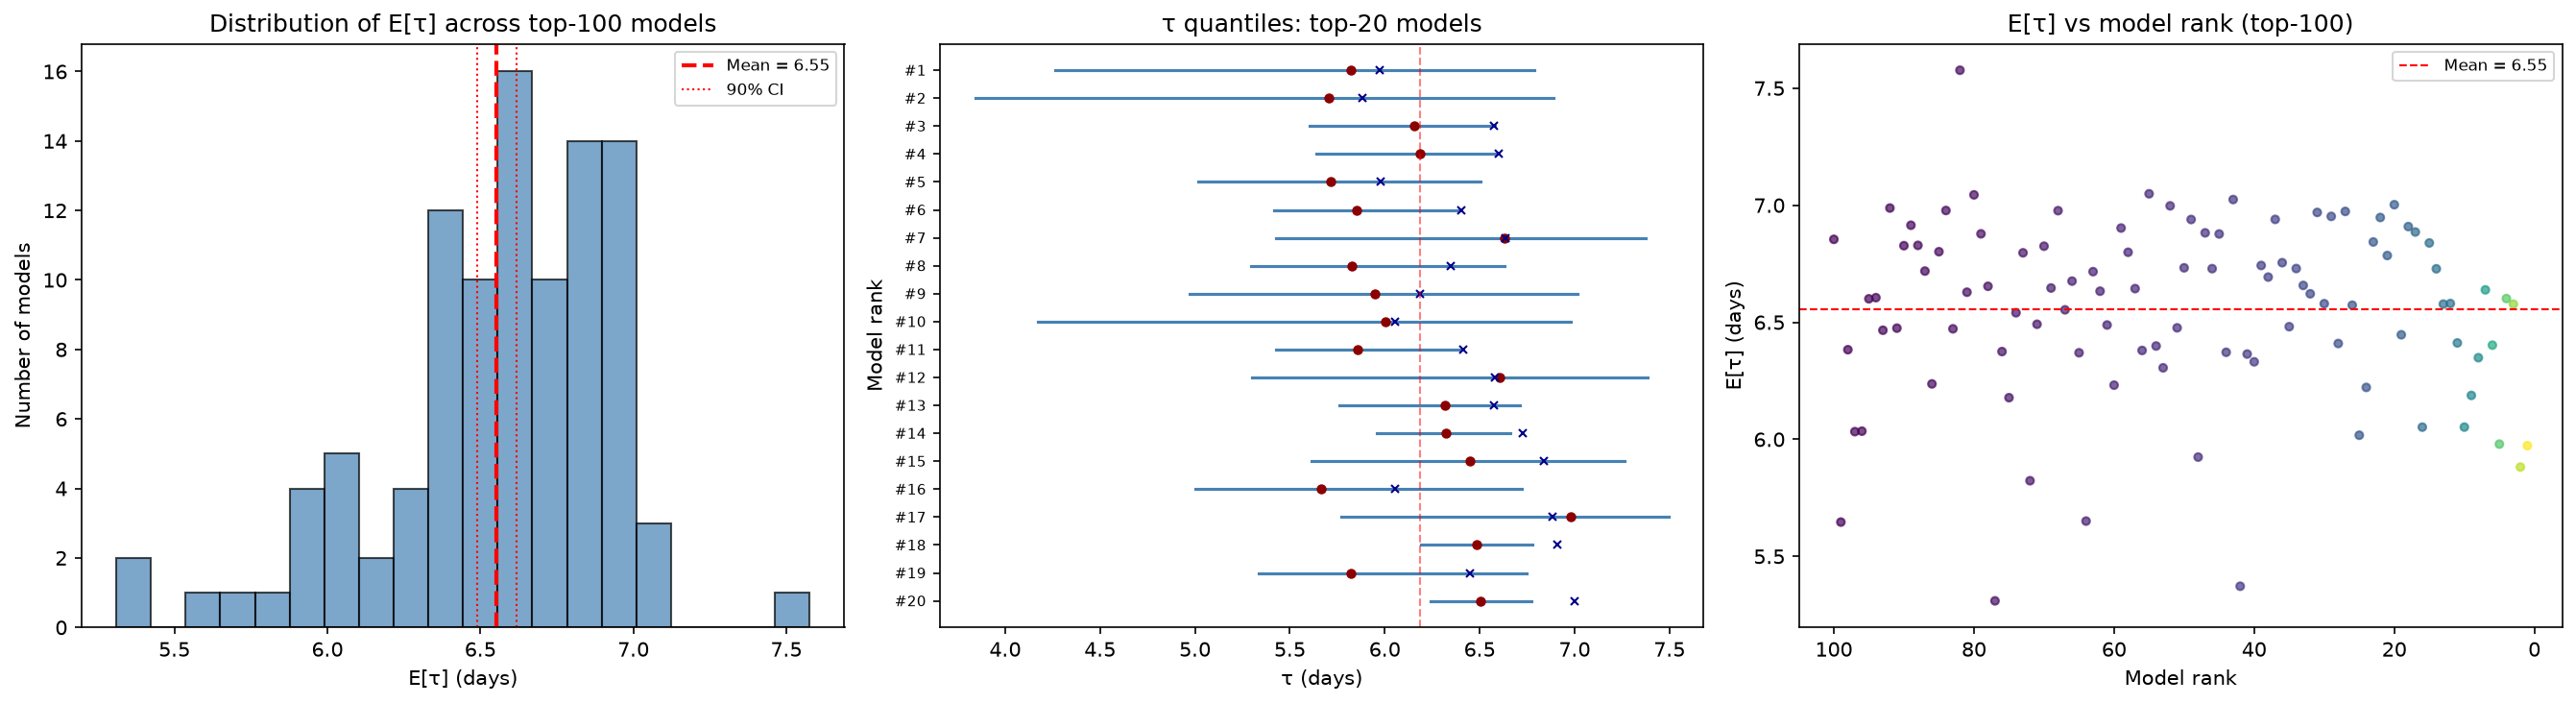
\includegraphics[width=0.92\textwidth]{top100_tau_analysis.png}
  \caption{Апостериорные характеристики $\tau$ для лучших конфигураций
  $896$-сетки: устойчивость onset при вариации ELPD и числа признаков.}
  \label{fig:top100-tau}
\end{figure*}

\begin{table}[t]
\centering
\caption{Апостериорные характеристики $\tau$ по квартилям ELPD
($896$-сетка $W/S$).}
\label{tab:tau-q}
\small
\begin{tabular}{lrrr}
\toprule
Квартиль & $\mathbb{E}[\tau]$ & $Q_2(\tau)$ & $\mathrm{std}$\\
\midrule
Q1 (лучшие) & $6{,}64\pm0{,}42$ & $6{,}27$ & $0{,}88$\\
Q2 & $6{,}71\pm0{,}56$ & $6{,}32$ & $0{,}71$\\
Q3 & $6{,}54\pm0{,}70$ & $6{,}15$ & $0{,}81$\\
Q4 (худшие) & $6{,}46\pm0{,}88$ & $6{,}19$ & $1{,}00$\\
\bottomrule
\end{tabular}
\end{table}

\subsection{Ранжирование признаков зависит от сетки}

В $896$-сетке верхний квартиль доминирует \texttt{concat:mean}
(Student-$t$, окно~$2$\,ч; $94\%$ моделей Q1). В июльской сетке верхние
позиции занимает \texttt{daily:range} с plain~Beta, затем
\texttt{daily:mean+range}; доминирует разрешение $N{=}48$,
$\mathrm{ov}{=}0$. Это \emph{не} основание объявлять единственного
``победителя'': разные онтологии признаков и likelihood несопоставимы
как физиологический ранг без контроля артефактов.

\begin{figure}[t]
  \centering
  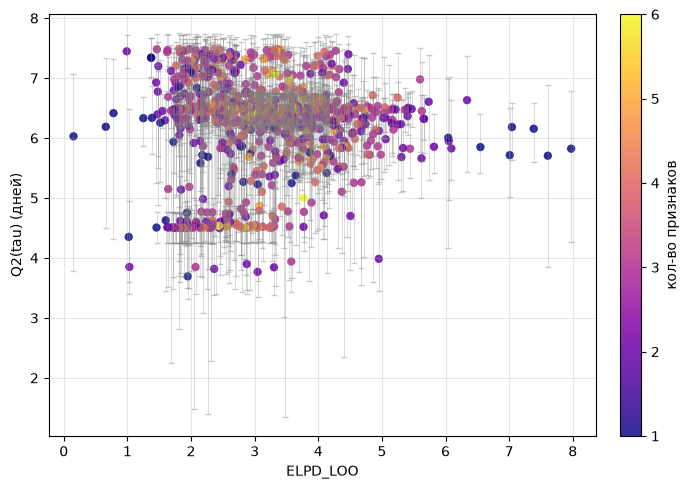
\includegraphics[width=\linewidth]{q2_tau.png}
  \caption{Медиана апостериорного $Q_2(\tau)$ vs ELPD-LOO
  ($896$-сетка). Усы --- $[Q_1(\tau),Q_3(\tau)]$.}
  \label{fig:q2-tau}
\end{figure}

\subsection{Граница Beta и размах: почему plain beta отвергнут}

После масштабирования $R/2$ около $25$--$30\%$ суточных значений
размаха лежат в $[0{,}9,\,1]$ (при $N{=}48$ --- до $\approx0{,}30$;
массы у $0$ нет). Апостериоры top-моделей тянут $\beta\ll 1$
(типично $\beta_1\approx 0{,}5$--$0{,}7$ при prior $\Gamma(\mu{=}3,
\sigma{=}1{,}5)$, дающем лишь $\sim 5\%$ массы ниже $1$), а
поточечный log-lik коррелирует с близостью $y$ к~$1$
($r\approx 0{,}8$--$0{,}9$) --- сигнатура boundary blow-up, а не
плоского выигрыша в fit.

\begin{table}[t]
\centering
\caption{Smoke: plain beta vs constrained / IIB
($N{=}48$, $\mathrm{ov}{=}0$; daily:range).}
\label{tab:beta-smoke}
\small
\begin{tabular}{lrrr}
\toprule
Модель & ELPD/$F E'$ & $\mathbb{E}[\tau]$ & $\mathrm{frac}(\beta{<}1)$\\
\midrule
plain beta & $6{,}62$ & $6{,}23$ & $\beta_1{:}1{,}00$\\
\texttt{beta\_constrained} & $5{,}18$ & $7{,}29$ & $0$\\
IIB@$0{,}9$ & $4{,}83$ & $7{,}29$ & $0$\\
mean+range + constr. & $5{,}26$ & $7{,}35$ & $0$\\
\bottomrule
\end{tabular}
\end{table}

Ограничение $\alpha,\beta\ge 1$ или IIB снимает $\sim\!1{,}4$ единицы
нормированного ELPD с лидера plain~beta, тогда как
$\mathbb{E}[\tau]$ остаётся в полосе $\sim 6$--$8$\,сут. После
ограничения scores range-only / mean+range ($\sim 5{,}2$) садятся
рядом с mean-only уровнями полной сетки ($\sim 5{,}4$--$5{,}7$), а не
далеко выше них. Следовательно доминирование
plain-beta~\texttt{daily:range} по ELPD --- в значительной мере
артефакт likelihood; для выводов предпочтительны
\texttt{beta\_constrained} / IIB, \texttt{daily:mean} или
\texttt{mean+range}. Положительный ELPD при этом остаётся
корректным log-score continuous densities.

\begin{figure}[t]
  \centering
  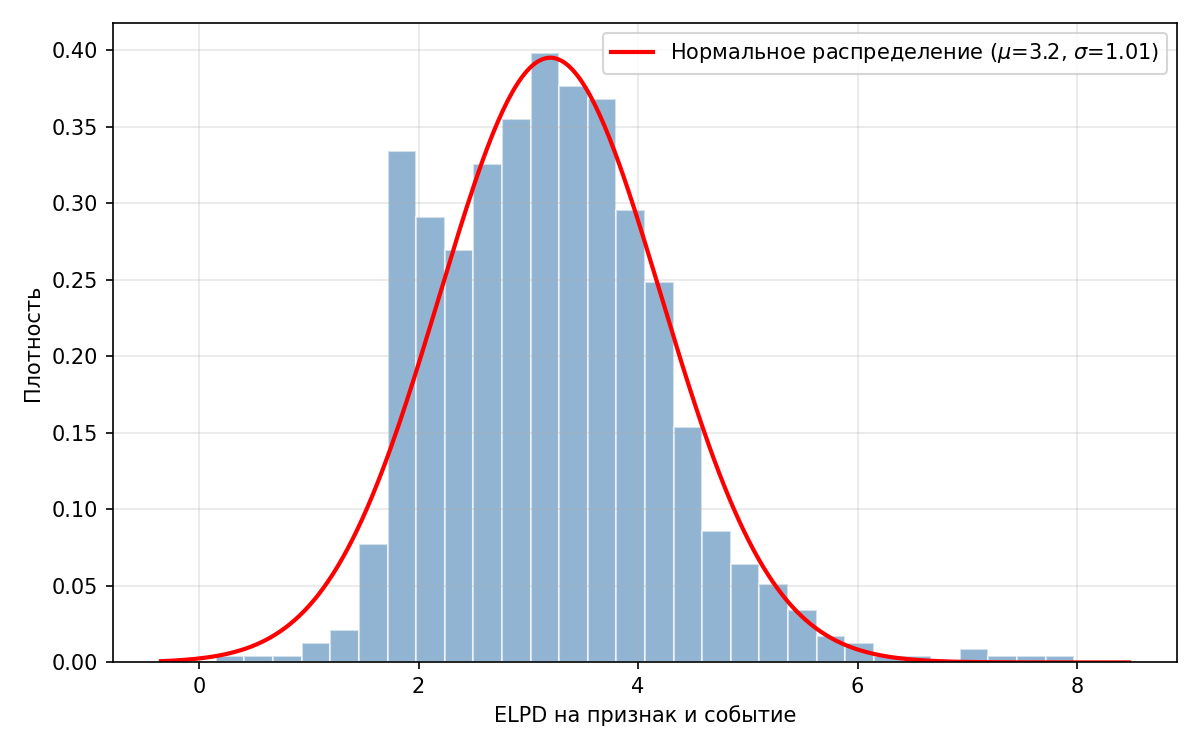
\includegraphics[width=\linewidth]{hist_elpd.png}
  \caption{Распределение нормированного ELPD по конфигурациям
  $896$-сетки: плато массы и верхний хвост лидеров.}
  \label{fig:hist-elpd}
\end{figure}

\subsection{Связь с классическим окном $2$--$4$ суток}

Классические тесты по размаху профиля ПС ($N{=}12$, $\mathrm{ov}{=}0$)
фиксируют момент, когда отклонение становится большим относительно
тихих контролей ($\sim 2$--$4$\,сут до/после; сильнейшее
послесобытийное искажение часто на $+1\ldots+3$, пресобытийный
эффект наиболее ясен на $-2,-1$). Пороговые правила краткосрочного
прогноза в той же линии опирались на изменения REM за $\sim 3$ суток.
Байесовский $\tau\sim 6{,}6$ оценивает более ранний onset режима.
Оценки совместимы, если эффект нарастает несколько суток, но это
\emph{разные} параметры: нельзя ``опровергать'' классику байесовским
$\tau$ и наоборот. Июльский акцент на daily-range ближе к классической
доктрине, чем диссертационный фаворит \texttt{concat:mean} --- при
условии density-safe likelihood.

\subsection{Чувствительность и протокол чистоты}

Протокол integrity фиксирует primary-конфиги \emph{до} нарративов
ранжирования:
\begin{itemize}[leftmargin=1.3em,itemsep=0.2em,topsep=0.3em]
  \item \textbf{Primary A} (мост к диссертации):
  \texttt{daily:mean+range}, $N{=}24$, $\mathrm{ov}{=}0{,}5$
  ($\equiv W{=}2,S{=}1$), mean student\_t/normal + range
  \texttt{beta\_constrained}/IIB;
  \item \textbf{Primary B}: \texttt{daily:range} с
  \texttt{beta\_constrained}/IIB на тройке $(N,\mathrm{ov})\in
  \{(48,0),(48,0{,}25),(24,0{,}5)\}$ --- отчёт по всем трём, без
  cherry-pick.
\end{itemize}
Plain beta --- только диагностический контраст boundary-аудита.
Явно не primary: shape\_shift / L1--L2, half-day без daily-агрегатов,
кросс-builder ELPD vs CSV~$896$.

Страты чувствительности: before-only vs full (before +
after\_reversed); arm без $2024$-$09$-$30$; маскирование артефактных
суток (каноническая карта: R2~$2022$-$11$-$07$ day~$0$; R2/R3
$2023$-$05$-$03$ day~$2$; R2~$2023$-$04$-$21$ after\_reversed day~$3$).
Негативный контроль: \texttt{shuffle\_dates} (внутри крысы) /
\texttt{permute\_labels} (глобально) с тем же builder'ом; при нуле
ожидают сдвиг $\mathbb{E}[\tau]$ к центру prior ($\approx 5{,}5$),
уширение HDI и ухудшение ELPD относительно real-date primary. Dry-run
протокола (смена $78\%$ дат при seed~$0$) реализован; полный MCMC
null --- confirmatory-шаг.

Таблица чувствительности $\mathbb{E}[\tau]$ по
feature${}\times{}$likelihood${}\times{}N$ заполняется одним builder'ом
и бюджетом MCMC; ячейки с схлопыванием к краям prior ($\approx 3$ или
$\approx 8$) помечают как неидентифицируемые и не усредняют вслепую.
Уже доступный smoke ($N{=}48$, $\mathrm{ov}{=}0$) даёт диапазон
$\mathbb{E}[\tau]\approx 6{,}2$--$7{,}7$ при смене plain/constrained/IIB.

\section{Обсуждение и ограничения}

Выборка мала и неоднородна; модель допускает одну скачкообразную
разладку. Более сложные варианты --- плавный переход, несколько
точек, иерархия по животным/событиям --- требуют расширения данных.
Сравнивать абсолютные ELPD между старым observation builder и июльским
нельзя без общего конвейера. Токсичные профили и неполные
\texttt{after\_reversed} должны быть явными стратами, а не тихим
фильтром.

Для топ-$10$ моделей $896$-сетки не выявлено записей с
$\hat k\ge 0{,}7$ ($\Delta\elpd{=}0$ после возможного исключения) ---
внутри этой сетки лидеры не держатся на одном экстремальном событии.
В июле, напротив, R2/R3~$2024$-$09$-$30$ систематически Pareto-тяжёлые;
shape-блок каждый раз дропает R2. Это подчёркивает: робастность $\tau$
не отменяет гигиены токсичных окон.

Интерпретация консервативна: изменение REM-ассоциированного состояния,
а не доказательство стресса и не сейсмический прогноз. Перспектива ---
проспективная фиксация primary-конфига на новых событиях; сопоставление
силы эффекта с магнитудой, глубиной и дистанцией; полный MCMC
негативного контроля; заполнение таблицы чувствительности
$\mathbb{E}[\tau]$ по feature${}\times{}$likelihood${}\times{}N$.

\section{Выводы}

\begin{enumerate}[leftmargin=1.2em,itemsep=0.35em]
  \item Байесовская модель одной точки разладки с маргинализацией $\tau$
  устойчиво локализует смену REM-режима на $\mathbb{E}[\tau]\approx
  6{,}5$--$6{,}7$ суток до события при двух сетках предобработки.
  \item Ранг признаков по LOO зависит от сетки и likelihood; нельзя
  утверждать уникальность \texttt{concat:mean} или plain-beta
  \texttt{daily:range} без оговорок.
  \item Для размаха профиля ПС plain~Beta у границы~$1$ завышает ELPD;
  предпочтительны constrained~beta / IIB / mean+range.
  \item Классическое окно эффекта $2$--$4$\,сут и байесовский onset
  $\tau\sim 6{,}6$ --- разные estimand'ы; терминология согласована с
  прежними отчётами ($12\times 2$\,ч, размах профиля ПС).
  \item Протокол чистоты (primary-конфиги, страты токсичных окон,
  негативный контроль) задаёт рамку для confirmatory-прогонов.
\end{enumerate}

\begin{ack}
Работа опирается на данные непрерывной регистрации сна на Камчатке и
программный конвейер \texttt{seismic-pipeline}. Автор благодарен
коллегам по нейросейсмологическим измерениям за доступ к гипнограммам
и обсуждение классических протоколов размаха профиля ПС.
\end{ack}

{\small
\bibliographystyle{plainnat}
\bibliography{references}
}

\end{document}
